% Created by tikzDevice version 0.12.3 on 2019-11-29 23:49:46
% !TEX encoding = UTF-8 Unicode
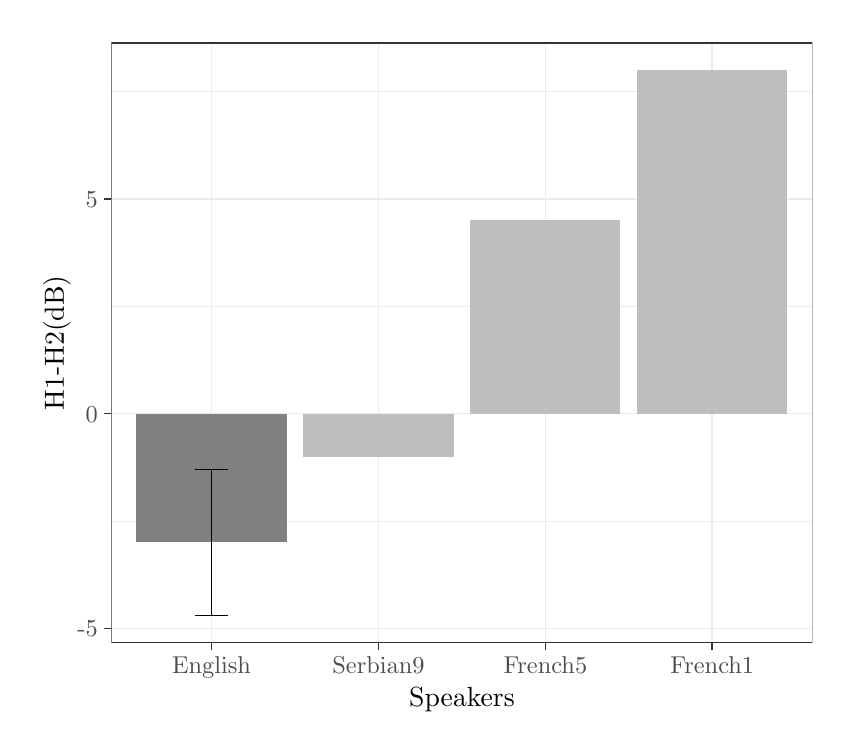
\begin{tikzpicture}[x=1pt,y=1pt]
\definecolor{fillColor}{RGB}{255,255,255}
\path[use as bounding box,fill=fillColor,fill opacity=0.00] (0,0) rectangle (289.08,252.94);
\begin{scope}
\path[clip] (  0.00,  0.00) rectangle (289.08,252.94);
\definecolor{drawColor}{RGB}{255,255,255}
\definecolor{fillColor}{RGB}{255,255,255}

\path[draw=drawColor,line width= 0.6pt,line join=round,line cap=round,fill=fillColor] (  0.00,  0.00) rectangle (289.08,252.94);
\end{scope}
\begin{scope}
\path[clip] ( 30.25, 30.69) rectangle (283.58,247.45);
\definecolor{fillColor}{RGB}{255,255,255}

\path[fill=fillColor] ( 30.25, 30.69) rectangle (283.58,247.45);
\definecolor{drawColor}{gray}{0.92}

\path[draw=drawColor,line width= 0.3pt,line join=round] ( 30.25, 74.67) --
	(283.58, 74.67);

\path[draw=drawColor,line width= 0.3pt,line join=round] ( 30.25,152.25) --
	(283.58,152.25);

\path[draw=drawColor,line width= 0.3pt,line join=round] ( 30.25,229.83) --
	(283.58,229.83);

\path[draw=drawColor,line width= 0.6pt,line join=round] ( 30.25, 35.88) --
	(283.58, 35.88);

\path[draw=drawColor,line width= 0.6pt,line join=round] ( 30.25,113.46) --
	(283.58,113.46);

\path[draw=drawColor,line width= 0.6pt,line join=round] ( 30.25,191.04) --
	(283.58,191.04);

\path[draw=drawColor,line width= 0.6pt,line join=round] ( 66.44, 30.69) --
	( 66.44,247.45);

\path[draw=drawColor,line width= 0.6pt,line join=round] (126.75, 30.69) --
	(126.75,247.45);

\path[draw=drawColor,line width= 0.6pt,line join=round] (187.07, 30.69) --
	(187.07,247.45);

\path[draw=drawColor,line width= 0.6pt,line join=round] (247.39, 30.69) --
	(247.39,247.45);
\definecolor{fillColor}{gray}{0.50}

\path[fill=fillColor] ( 39.29, 66.92) rectangle ( 93.58,113.46);
\definecolor{fillColor}{RGB}{190,190,190}

\path[fill=fillColor] ( 99.61, 97.95) rectangle (153.90,113.46);

\path[fill=fillColor] (159.93,113.46) rectangle (214.21,183.29);

\path[fill=fillColor] (220.25,113.46) rectangle (274.53,237.59);
\definecolor{drawColor}{RGB}{0,0,0}

\path[draw=drawColor,line width= 0.6pt,line join=round] ( 60.40, 93.29) --
	( 72.47, 93.29);

\path[draw=drawColor,line width= 0.6pt,line join=round] ( 66.44, 93.29) --
	( 66.44, 40.54);

\path[draw=drawColor,line width= 0.6pt,line join=round] ( 60.40, 40.54) --
	( 72.47, 40.54);

\definecolor{drawColor}{gray}{0.20}

\path[draw=drawColor,line width= 0.6pt,line join=round,line cap=round] ( 30.25, 30.69) rectangle (283.58,247.45);
\end{scope}
\begin{scope}
\path[clip] (  0.00,  0.00) rectangle (289.08,252.94);
\definecolor{drawColor}{gray}{0.30}

\node[text=drawColor,anchor=base east,inner sep=0pt, outer sep=0pt, scale=  0.88] at ( 25.30, 32.85) {-5};

\node[text=drawColor,anchor=base east,inner sep=0pt, outer sep=0pt, scale=  0.88] at ( 25.30,110.43) {0};

\node[text=drawColor,anchor=base east,inner sep=0pt, outer sep=0pt, scale=  0.88] at ( 25.30,188.01) {5};
\end{scope}
\begin{scope}
\path[clip] (  0.00,  0.00) rectangle (289.08,252.94);
\definecolor{drawColor}{gray}{0.20}

\path[draw=drawColor,line width= 0.6pt,line join=round] ( 27.50, 35.88) --
	( 30.25, 35.88);

\path[draw=drawColor,line width= 0.6pt,line join=round] ( 27.50,113.46) --
	( 30.25,113.46);

\path[draw=drawColor,line width= 0.6pt,line join=round] ( 27.50,191.04) --
	( 30.25,191.04);
\end{scope}
\begin{scope}
\path[clip] (  0.00,  0.00) rectangle (289.08,252.94);
\definecolor{drawColor}{gray}{0.20}

\path[draw=drawColor,line width= 0.6pt,line join=round] ( 66.44, 27.94) --
	( 66.44, 30.69);

\path[draw=drawColor,line width= 0.6pt,line join=round] (126.75, 27.94) --
	(126.75, 30.69);

\path[draw=drawColor,line width= 0.6pt,line join=round] (187.07, 27.94) --
	(187.07, 30.69);

\path[draw=drawColor,line width= 0.6pt,line join=round] (247.39, 27.94) --
	(247.39, 30.69);
\end{scope}
\begin{scope}
\path[clip] (  0.00,  0.00) rectangle (289.08,252.94);
\definecolor{drawColor}{gray}{0.30}

\node[text=drawColor,anchor=base,inner sep=0pt, outer sep=0pt, scale=  0.88] at ( 66.44, 19.68) {English};

\node[text=drawColor,anchor=base,inner sep=0pt, outer sep=0pt, scale=  0.88] at (126.75, 19.68) {Serbian9};

\node[text=drawColor,anchor=base,inner sep=0pt, outer sep=0pt, scale=  0.88] at (187.07, 19.68) {French5};

\node[text=drawColor,anchor=base,inner sep=0pt, outer sep=0pt, scale=  0.88] at (247.39, 19.68) {French1};
\end{scope}
\begin{scope}
\path[clip] (  0.00,  0.00) rectangle (289.08,252.94);
\definecolor{drawColor}{RGB}{0,0,0}

\node[text=drawColor,anchor=base,inner sep=0pt, outer sep=0pt, scale=  1.00] at (156.91,  7.64) {Speakers};
\end{scope}
\begin{scope}
\path[clip] (  0.00,  0.00) rectangle (289.08,252.94);
\definecolor{drawColor}{RGB}{0,0,0}

\node[text=drawColor,rotate= 90.00,anchor=base,inner sep=0pt, outer sep=0pt, scale=  1.00] at ( 13.08,139.07) {H1-H2(dB)};
\end{scope}
\end{tikzpicture}
